\documentclass[a4paper,11pt,UTF8]{article}
\usepackage{ctex}
\usepackage{amsmath,amsthm,amssymb,amsfonts}
\usepackage{amsmath}
\usepackage[a4paper]{geometry}
\usepackage{graphicx}
\usepackage{microtype}
\usepackage{siunitx}
\usepackage{booktabs}
\usepackage[colorlinks=false, pdfborder={0 0 0}]{hyperref}
\usepackage{cleveref}
\usepackage{esint} 
\usepackage{graphicx}
\usepackage{ragged2e}
\usepackage{pifont}
\usepackage{extarrows}
\title{}
\author{}

\begin{document}
\noindent
6.Solution :\\
(1)以D点为原点,以$\overrightarrow{DA},\overrightarrow{DC},\overrightarrow{DP}$为$x,y,z$轴正方向,建立空间直角坐标系$D-xyz$\\
设$\displaystyle PD=DC=1\Rightarrow\overrightarrow{FE}=\{\frac{1}{2},0,-\frac{1}{2}\},\overrightarrow{DC}=\{0,1,0\}$\\
$\because\overrightarrow{FE}\cdot\overrightarrow{DC}=0\\\therefore FE\perp  DC$\\
(2)设$\displaystyle G(a,0,c)\Rightarrow\overrightarrow{GF}=\{\frac{1}{2}-a,\frac{1}{2},\frac{1}{2}-c\}$\\
$\overrightarrow{PC}={0,1,-1},\overrightarrow{CB}={1,0,0}$\\
设$\mathbf{n}=\{x,y,z\}$为面$PCB$的一个法向量\\
$\begin{cases}
	\overrightarrow{PC}\cdot\mathbf{n}=0\\
	\overrightarrow{CB}\cdot\mathbf{n}=0
\end{cases}\Rightarrow
\begin{cases}
	y-z=0\\
	x=0
\end{cases}
$\\
$\Rightarrow\text{令}y=1,\text{得}\mathbf{n}=\{0,1,1\}$\\
$\because GF\perp \text{面}PCB\therefore GF//\mathbf{n}\Rightarrow\overrightarrow{GF}=\lambda\mathbf{n}$\\
$\begin{cases}
	...\\
	...
\end{cases}$\\
$\displaystyle\Rightarrow a=\frac{1}{2}, c=0$\\
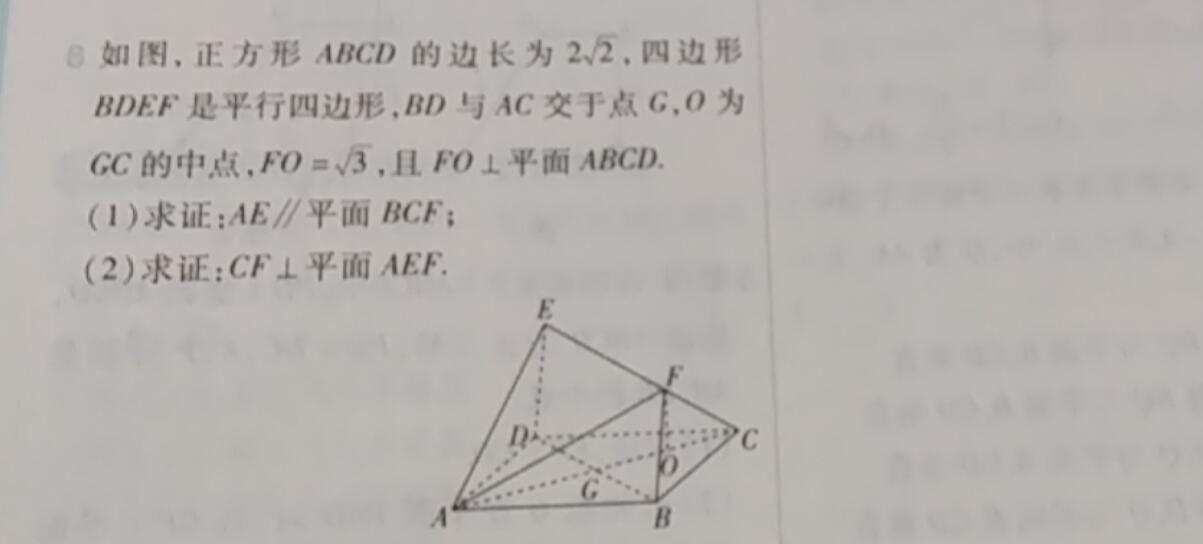
\includegraphics[scale=0.5]{./P14T8.jpg}\\
8.Solution\\
(1)\\
易知:$DE//BF,AD//BC$\\
$\because DE\nsubseteq BFC,BF\subset BFC,AD\nsubseteq BFC,BC\subset BFC$\\
$\therefore AD,DE//BFC$\\
$\because\begin{cases}
	AD,DE//BFC\\
	AD,DE\nsubseteq BFC\\
	AD\cap DE=D\\
\end{cases}\Rightarrow ADE//BFC$\\
$\because AE\subset ADE\therefore AE//ADE$
(2)取$BC$中点为$M$,以O点为原点,以$\overrightarrow{OA},\overrightarrow{OM},\overrightarrow{OF}$为$x,y,z$轴正方向,建立空间直角坐标系$O-xyz$\\
$\therefore \overrightarrow{AF}=\{-3,0,\sqrt{3}\},\overrightarrow{EF}=\{0,4,0\},\overrightarrow{CF}=\{1,0,\sqrt{3}\}$\\
设$\mathbf{n}=\{x,y,z\}$为面$AEF$的一个法向量\\
$\begin{cases}
	\overrightarrow{AF}\cdot\mathbf{n}=0\\
	\overrightarrow{EF}\cdot\mathbf{n}=0
\end{cases}\Rightarrow
\begin{cases}
	-3x+\sqrt{3}z=0\\
	y=0
\end{cases}
$\\
$\Rightarrow\text{令}z=\sqrt{3},\text{得}\mathbf{n}=\{1,0,\sqrt{3}\}$\\
$\because \overrightarrow{CF}=\mathbf{n}\\\therefore CF\perp AEF$\\
9.Solution\\
$\text{证明}:(1)\because DE\bot AB,BE\perp DE\\
\text{又}\because BE\bot A_1D,
DE\cap A_{1}D=D\\
\therefore BE\bot\text{平面}A_1DE\\
\because A_1E\subset\text{平面}A_1DE,\\ \therefore A_1E\bot BE\\
\text{又}A_1E\bot DE,BE \cap DE= E\\
\therefore A_1E\bot\text{平面}BCDE$\\
(2)
$\because A_{1}E\bot $平面$BCDE$,$BE\bot DE$\\
$\therefore$以$E$为坐标原点,分别以$\overrightarrow{EB},\overrightarrow{ED},\overrightarrow{EA}$所在方向为$x,y,z$轴正方向,建立空间直角坐标系$E-xyz$\\$
\text{则}B\left(1,0,0\right),\:D(0:,\sqrt3,\:0),\:A_1(0,0,1)
\overrightarrow{BA_1}=(-1,0,1)\:,\:\overrightarrow{BD}=(-1,\sqrt{3},0)\\
\text{设平面}A_1BD\text{的法向量为}\overrightarrow{n}=(x,y,z)\text{,}
\text{由}\left\{\begin{array}{ll}\overrightarrow{n}\cdot\overrightarrow{BA_1}=-x+z=0\\\overrightarrow{n}\cdot\overrightarrow{BD}=-x+\sqrt{3}y=0\end{array}\right.\\
\Rightarrow\text{取}y=1\text{,得}\overrightarrow{n}=(\sqrt{3}\:,\:1\:,\:\sqrt{3})$.\\
假设在线段$BD$上存在一点$P$,使得平面$A_1EP\bot$平面$A_1BD$.\\
设$P(a,b,0),BP =\lambda BD(0\leq\lambda<1)$,则:\\
$
(a-1,b,0)=\lambda(-1\:,\:\sqrt{3}\:,\:0)
$
$\Rightarrow a = 1-\lambda,b= \sqrt{3}\lambda\Rightarrow P(1-\lambda,\sqrt{3}\lambda,0)$\\
$\therefore EA_1 =(0,0,1),EF =(1-\lambda,\sqrt{3}\lambda,0)$.设平面$A,EP$的法向量$m =(x_1,y_1,z_1)$,\\
$\begin{cases}
	\overrightarrow { m }\cdot\overrightarrow{EA_1}=z_1=0\\
	\overrightarrow{m}\cdot\overrightarrow{EP}=(1-\lambda)x_{1}+\sqrt{3}\lambda y_{1}=0
\end{cases}$\\
$\Rightarrow$取
$
x_1=\sqrt{3}\lambda,\text{得}\overrightarrow{m}=(\sqrt{3}\lambda,\lambda-1,0)
$\\
$\because\text{平面}A_1EP\bot\text{平面}A_1BD~,\text{得}$
$\overrightarrow{m}\cdot\overrightarrow{n}=3\lambda+\lambda-1=0$,解得$\displaystyle\lambda=\frac{1}{4}$\\
$\therefore$在线段$BD$上存在点$P$,使得平面$\displaystyle A_1EP\bot$平面$\displaystyle A_{1}BD,\text{且}\frac{BP}{BD}=\frac{1}{4}.$\\\\
P16T6:\\
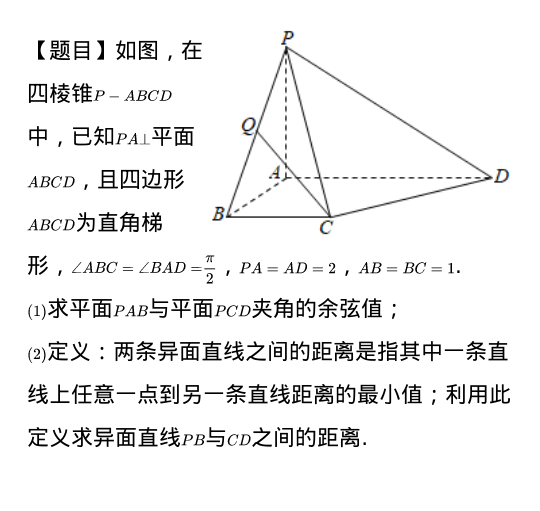
\includegraphics[scale=0.5]{./P16T6.jpg}\\
Solution:\\
(1)\\
$\because AP\bot $平面$ABCD$,$AB\bot AD$\\
$\therefore$以$A$为坐标原点,分别以$\overrightarrow{AB},\overrightarrow{AD},\overrightarrow{AP}$所在方向为$x,y,z$轴正方向,建立空间直角坐标系$A-xyz$\\
$\therefore \overrightarrow{PD}=\{0,2,-2\},\overrightarrow{CD}=\{-1,1,0\}$\\
易知$\overrightarrow{AD}=\{0,2,0\}$为面 $APB$的一个法向量(你要写证明过程)\\
设 $\overrightarrow{n}=\{x,y,z\}$为面$PCD$的一个法向量\\
$\begin{cases}
	\overrightarrow{PD}\cdot\mathbf{n}=0\\
	\overrightarrow{CD}\cdot\mathbf{n}=0
\end{cases}\Rightarrow
\begin{cases}
	2y-2z=0\\
	-x+y=0
\end{cases}
$\\
$\Rightarrow\text{令}x=1,\text{得}\mathbf{n}=\{1,1,1\}$\\
$\cos\theta=\cos<\overrightarrow{AD},\overrightarrow{n}>=\frac{\sqrt{3}}{3}$\\
(2)\\
$\displaystyle
\text{因为}\overrightarrow{BP}=\left(-1,0,2\right), 
\text{设}\overrightarrow{BQ}=\lambda\overrightarrow{BP}=\left(\lambda,0,2\lambda\right),$ \\
$\displaystyle\text{又}\overrightarrow{CD}=\left(-1,1,0\right), 
\text{则}\overrightarrow{CQ}=\overrightarrow{CB}+\overrightarrow{BQ}=\begin{pmatrix}-\lambda,-1,2\lambda\end{pmatrix}, \\$
$\displaystyle\text{所以} 
d=\sqrt{\overrightarrow{CQ}^2-(\frac{\overrightarrow{CQ}\bullet\overrightarrow{CD}}{|\overrightarrow{CD}|})^2} 
=\sqrt{\frac92\lambda^2+\lambda+\frac12}=\sqrt{\frac92(\lambda+\frac19)^2+\frac49} \geq\sqrt{\frac49}=\frac23, \\
\text{所以异面直线}PB\text{与}CD\text{之间的距离}\frac23.\\
$
P16T7:\\
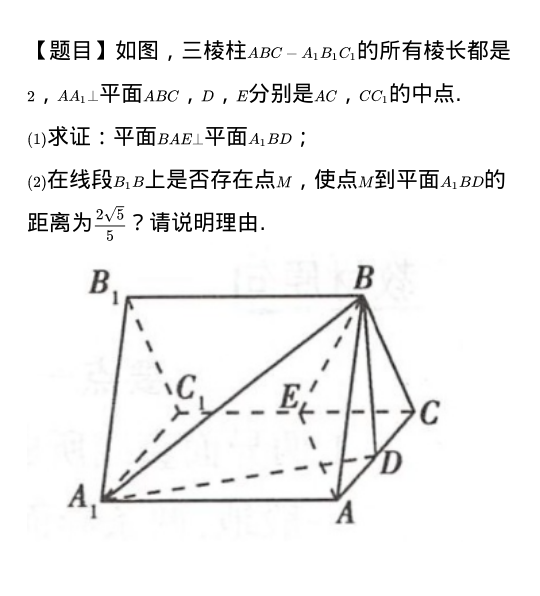
\includegraphics[scale=0.5]{./P16T7.jpg}\\
Solution:\\
取 $A_{1}C_{1}$ 的中点 $\text{0}$ 连接 $B_1O,OD\:,$易得 $OA_1,OD,OB_1$ 两两垂直.以$O$为坐标原点,分别以$\overrightarrow{OA_1},\overrightarrow{OD},\overrightarrow{OB_1}$所在方向为$x,y,z$轴正方向,建立空间直角坐标系$O-xyz$\\
(1) 证明: 易知 $\overrightarrow{A_1 D}=(-1,2,0), \overrightarrow{A_1 B}=(-1$, $2, \sqrt{3}), \overrightarrow{B A}=(1,0,-\sqrt{3}), \overrightarrow{B E}=(-1,-1$, $-\sqrt{3})$.\\
设 $\boldsymbol{n}_1=\left(x_1, y_1, z_1\right), \boldsymbol{n}_2=\left(x_2, y_2, z_2\right)$ 分别为 平面 $A_1 B D$ 和平面 $B A E$ 的法向量,\\
由 $\left\{\begin{array}{l}\overrightarrow{A_1 D} \cdot \boldsymbol{n}_1=0, \\ \overrightarrow{A_1 B} \cdot \boldsymbol{n}_1=0\end{array}\right.$ 得 $\left\{\begin{array}{l}-x_1+2 y_1=0, \\ -x_1+2 y_1+\sqrt{3} z_1=0,\end{array}\right.$\\ 
令 $y_1=1$, 则 $x_1=2, z_1=0$,\\
$\therefore \boldsymbol{n}_1=(2,1,0)$ 是平面 $A_1 B D$ 的一个法 向量.\\
由 $\left\{\begin{array}{l}\overrightarrow{B A} \cdot \boldsymbol{n}_2=0, \\ \overrightarrow{B E} \cdot \boldsymbol{n}_2=0\end{array}\right.$ 得 $\left\{\begin{array}{l}x_2-\sqrt{3} z_2=0, \\ -x_2-y_2-\sqrt{3} z_2=0,\end{array}\right.$\\
 令 $z_2=1$, 则 $x_2=\sqrt{3}, y_2=-2 \sqrt{3}$,\\
$\therefore \boldsymbol{n}_2=(\sqrt{3},-2 \sqrt{3}, 1)$ 是平面 $B A E$ 的一个法 向量,\\
$\therefore \boldsymbol{n}_2 \cdot \boldsymbol{n}_1=0, \therefore$ 平面 $B A E \perp$ 平面 $A_1 B D$.\\
(2) 假设在线段 $B_1 B$ (含端点) 上存在点
$M$, 使点 $M$ 到平面 $A_1 B D$ 的距离为 $\frac{2 \sqrt{5}}{5}$,\\
设 $M(0, a, \sqrt{3})(0 \leqslant a \leqslant 2)$,
则 $\overrightarrow{B M}=(0, a-2,0)$,\\
由 $\displaystyle \frac{2 \sqrt{5}}{5}=\frac{\left|\overrightarrow{B M} \cdot n_1\right|}{\left|n_1\right|}=\frac{|a-2|}{\sqrt{5}}$ 得 $a=4$ (舍去)
或 $a=0$,\\
故在线段 $B_1 B$ 上存在点 $M$, 即点 $M$ 与点 $B_1$ 重合时,
点 $M$ 到平面 $A_1 B D$ 的距离为 $\frac{2 \sqrt{5}}{5}$.\\
P16T7:\\
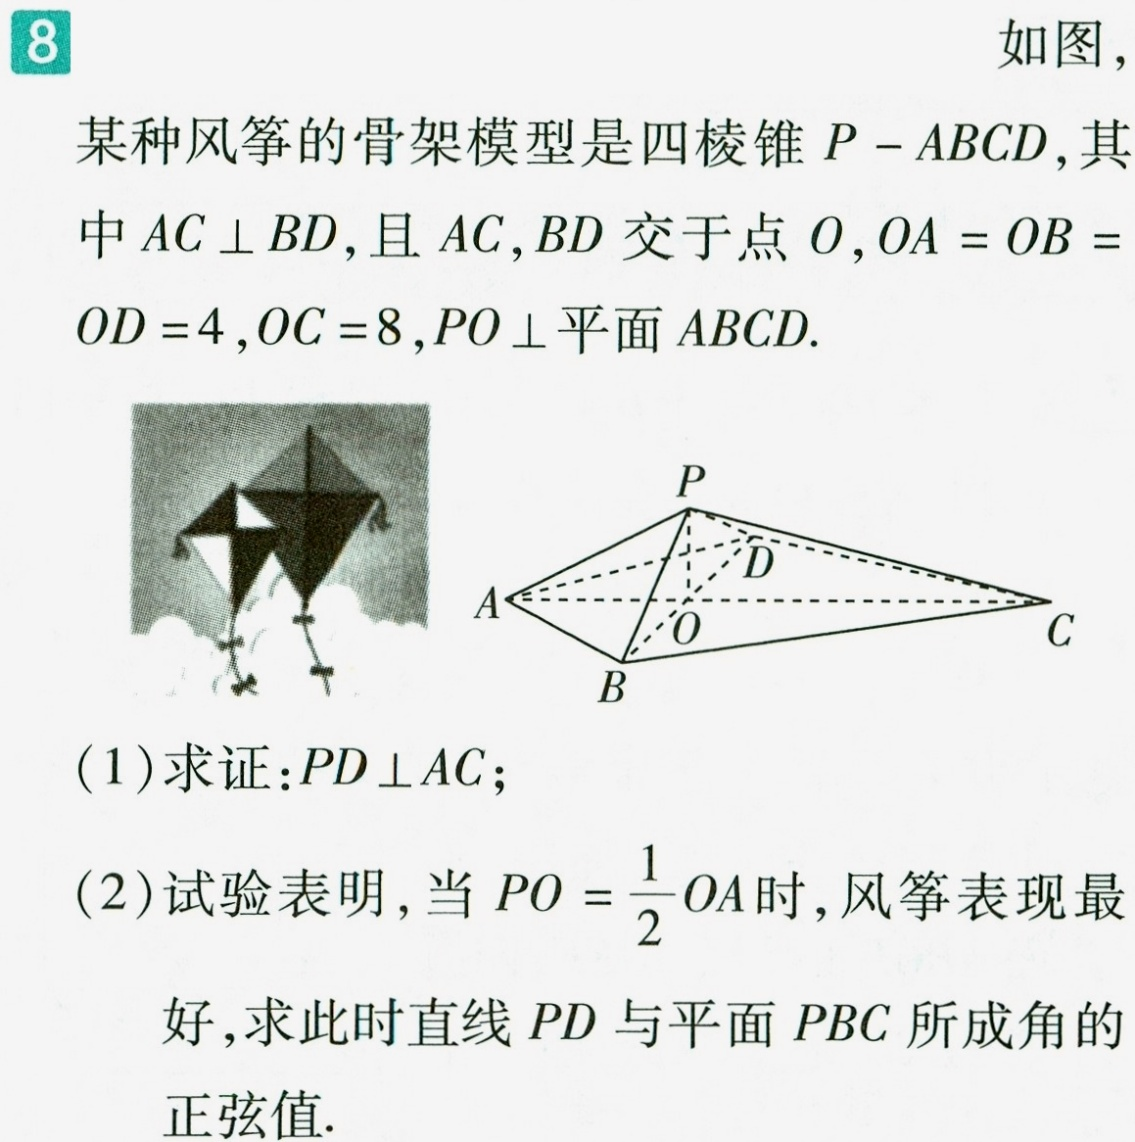
\includegraphics[scale=0.17]{./P18T9.jpg}\\
Solution:\\
8 (1) 因为 $P O \perp$ 平面 $A B C D, A C \subset$ 平面 $A B C D$, \\所以 $P O \perp A C$.\\
又 $A C \perp B D, P O \cap B D=O, P O \subset$ 平面 $P O D, B D \subset$ 平面 $P O D$, \\所以 $A C \perp$ 平面 $P O D$, 又 $P D \subset$ 平面 $P O D$,\\ 所以 $P D \perp A C$.\\
(2) 如图, 以 $O$ 为坐标原 点, 以 $\overrightarrow{O B}, \overrightarrow{O C}$, $\overrightarrow{O P}$ 的方向分别 为 $x, y, z$ 轴的正 方向, 建立空间直角坐标系 $O x y z$,\\
 则 $B(4,0,0)$, $C(0,8,0), D(-4,0,0), P(0,0,2)$,\\ 所以 $\overrightarrow{P B}=$ $(4,0,-2), \overrightarrow{P C}=(0,8,-2), \overrightarrow{P D}=(-4,0$, $-2)$.\\
设 $\boldsymbol{m}=(a, b, c)$ 为平面 $P B C$ 的法向量,\\
则 $\left\{\begin{array}{l}\boldsymbol{m} \cdot \overrightarrow{P B}=0 \\ \boldsymbol{m} \cdot \overrightarrow{P C}=0\end{array}\right.$, 即 $\left\{\begin{array}{l}4 a-2 c=0 \\ 8 b-2 c=0\end{array}\right.$,\\
取 $c=4$, 则 $\boldsymbol{m}=(2,1,4)$ 是平面 $P B C$ 的一个法 向量.\\
设直线 $P D$ 与平面 $P B C$ 所成角为 $\theta$,\\
则 $\displaystyle \sin \theta=\frac{|\overrightarrow{P D} \cdot m|}{|\overrightarrow{P D}||\boldsymbol{m}|}=\frac{16}{\sqrt{20} \times \sqrt{21}}=\frac{8 \sqrt{105}}{105}$.\\
P18T14:\\
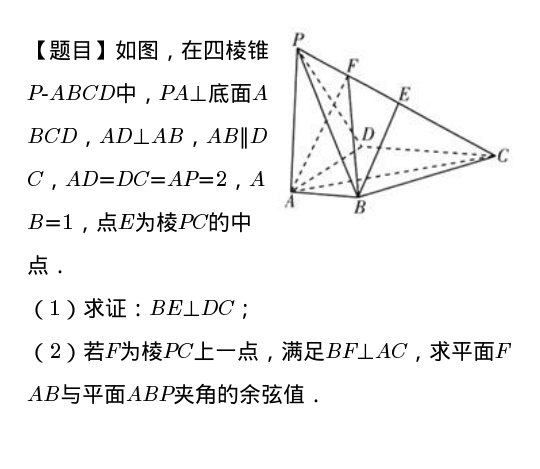
\includegraphics[scale=0.5]{./P18T14.jpg}\\
Solution:\\
(1)\\
(2)\\
P20T8:\\
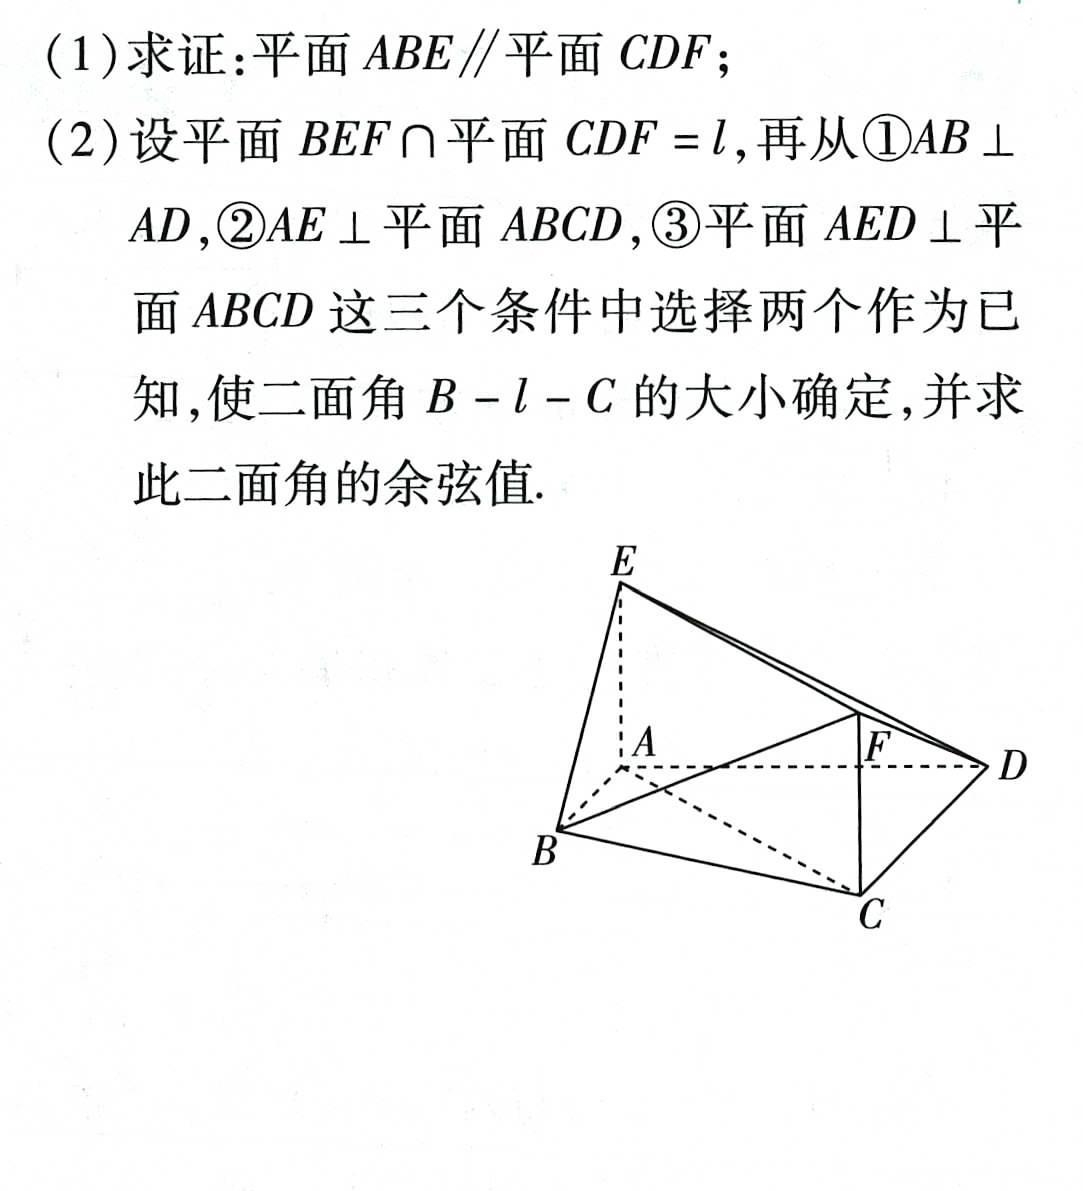
\includegraphics[scale=0.5]{./P20T8.jpg}\\
Solution:\\
(1)\\
(2)\\
P20T9:\\
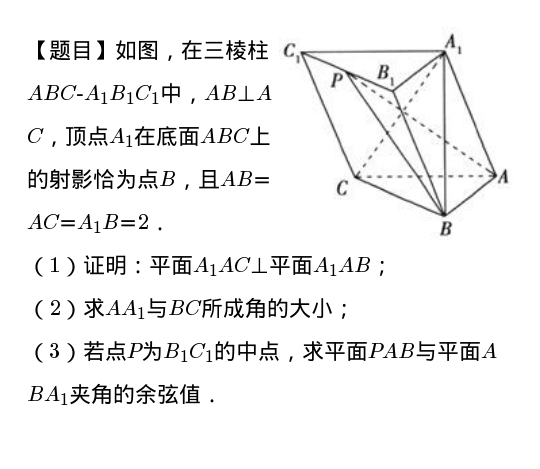
\includegraphics[scale=0.5]{./P20T9.jpg}\\
Solution:\\
(1)\\
(2)\\
P20T10:\\
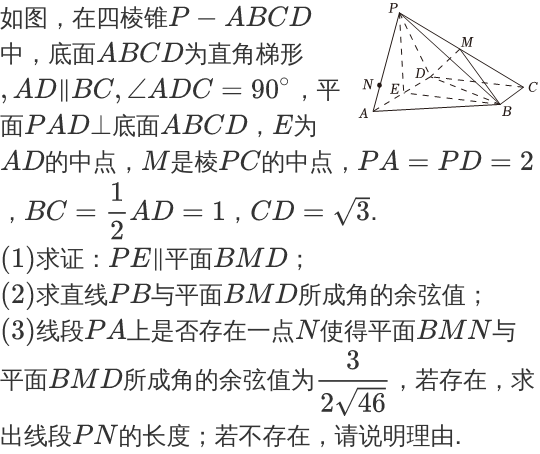
\includegraphics[scale=0.5]{./P20T10.jpg}\\
Solution:\\
(1)\\
(2)\\
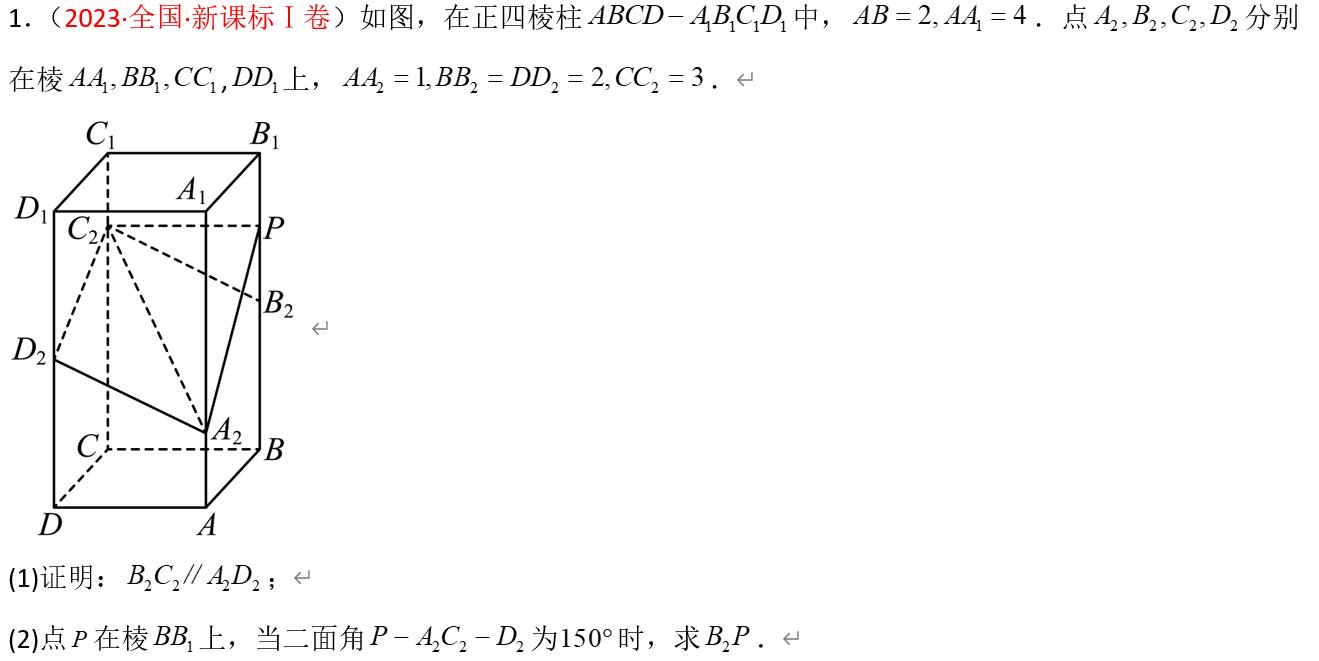
\includegraphics[scale=0.5]{./2023_new1.jpg}\\
Solution:\\
(1) 以 $C$ 为坐标原点, $C D, C B, C C_1$ 所在直线为 $x, y, z$ 轴建立空间直角坐标系,\\
则 $C(0,0,0), C_2(0,0,3), B_2(0,2,2), D_2(2,0,2), A_2(2,2,1)$,\\
$\therefore \overrightarrow{B_2 C_2}=(0,-2,1), \overrightarrow{A_2 D_2}=(0,-2,1)$,\\
$\therefore \overrightarrow{B_2 C_2} / / \overrightarrow{A_2 D_2}$,\\
又 $B_2 C_2, A_2 D_2$ 不在同一条直线上,\\
$\therefore B_2 C_2 / / A_2 D_2$.\\
(2) 设 $P(0,2, \lambda)(0 \leq \lambda \leq 4)$,\\
则 $\overrightarrow{A_2 C_2}=(-2,-2,2), \overrightarrow{P C_2}=(0,-2,3-\lambda), \overrightarrow{D_2 C_2}=(-2,0,1)$,\\
设平面 $P A_2 C_2$ 的法向量 $\vec{n}=(x, y, z)$,\\
则 $\left\{\begin{array}{l}\vec{n} \cdot \overrightarrow{A_2 C_2}=-2 x-2 y+2 z=0 \\ \vec{n} \cdot \overrightarrow{P C_2}=-2 y+(3-\lambda) z=0\end{array}\right.$,\\
令 $z=2$, 得 $y=3-\lambda, x=\lambda-1$,\\
$\therefore \vec{n}=(\lambda-1,3-\lambda, 2)$,\\
设平面 $A_2 C_2 D_2$ 的法向量 $\vec{m}=(a, b, c)$,\\
则 $\left\{\begin{array}{l}\vec{m} \cdot \overrightarrow{A_2 C_2}=-2 a-2 b+2 c=0 \\ \vec{m} \cdot \overrightarrow{D_2 C_2}=-2 a+c=0\end{array}\right.$,\\
令 $a=1$, 得 $b=1, c=2, \therefore \vec{m}=(1,1,2)$,\\
$\displaystyle\therefore|\cos \langle\vec{n}, \vec{m}\rangle|=\frac{|\vec{n} \cdot\\ \vec{m}|}{|\vec{n}||\vec{m}|}=\frac{6}{\sqrt{6}\\ \sqrt{4+(\lambda-1)^2+(3-\lambda)^2}}=\left|\cos 150^{\circ}\right|=\frac{\sqrt{3}}{2}$,\\
化简可得, $\lambda^2-4 \lambda+3=0$,\\
解得 $\lambda=1$ 或 $\lambda=3, \\\therefore P(0,2,1)$ 或 $P(0,2,3),  \\\therefore B_2 P=1$.\\
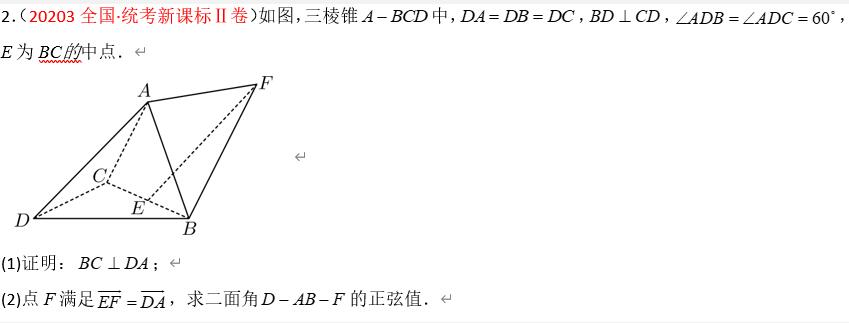
\includegraphics[scale=0.8]{./2023_new2.jpg}\\
Solution:\\
(1) 连接 $A E, D E$, 因为 $E$ 为 $B C$ 中点, $D B=D C$, 所以 $D E \perp B C$ (1),\\
因为 $D A=D B=D C, \angle A D B=\angle A D C=60^{\circ}$,\\ 所以 $\triangle A C D$ 与 $\triangle A B D$ 均为等边三角形, $\\\therefore A C=A B$, 从而 $A E \perp B C$ (2),\\ 由(1) (2), $A E \cap D E=E, A E, D E \subset$ 平面 $A D E$,\\
所以, $B C \perp$ 平面 $A D E$, 而 $A D \subset$ 平面 $A D E$, 所以 $B C \perp D A$.\\
(2) 不妨设 $D A=D B=D C=2, \because B D \perp C D, \therefore B C=2 \sqrt{2}, D E=A E=\sqrt{2}$.\\
$\therefore A E^2+D E^2=4=A D^2, \therefore A E \perp D E$, 又 $\because A E \perp B C, D E \cap B C=E, D E, B C \subset$ 平面 $B C D \therefore A E \perp$ 平面 $B C D$.
以点 $E$ 为原点, $E D, E B, E A$ 所在直线分别为 $x, y, z$ 轴, 建立空间直角坐标系, 如图所示:\\
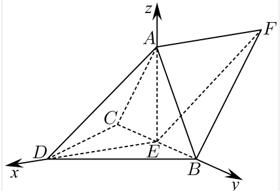
\includegraphics[scale=0.8]{./2023_new2s.jpg}\\
设 $D(\sqrt{2}, 0,0), A(0,0, \sqrt{2}), B(0, \sqrt{2}, 0), E(0,0,0)$,\\
设平面 $D A B$ 与平面 $A B F$ 的一个法向量分别为 $\overrightarrow{n_1}=\left(x_1, y_1, z_1\right), \overrightarrow{n_2}=\left(x_2, y_2, z_2\right)$,\\
二面角 $D-A B-F$ 平面角为 $\theta$, 而 $\overrightarrow{A B}=(0, \sqrt{2},-\sqrt{2})$,\\
因为 $\overrightarrow{E F}=\overrightarrow{D A}=(-\sqrt{2}, 0, \sqrt{2})$, 所以 $F(-\sqrt{2}, 0, \sqrt{2})$, 即有 $\overrightarrow{A F}=(-\sqrt{2}, 0,0)$,\\
$\therefore\left\{\begin{array}{l}-\sqrt{2} x_1+\sqrt{2} z_1=0 \\ \sqrt{2} y_1-\sqrt{2} z_1=0\end{array}\right.$,\\ 取 $x_1=1$, 所以 $\overrightarrow{n_1}=(1,1,1)$;\\
$\left\{\begin{array}{l}\sqrt{2} y_2-\sqrt{2} z_2=0 \\ -\sqrt{2} x_2=0\end{array}\right.$, 取 $y_2=1$, 所以 $\overrightarrow{n_2}=(0,1,1)$,\\
所以, $\displaystyle|\cos \theta|=\frac{\left|\vec{n}_1 \cdot \vec{n}_2\right|}{\left|\overrightarrow{n_1}\right|\left|\overrightarrow{n_2}\right|}=\frac{2}{\sqrt{3} \times \sqrt{2}}=\frac{\sqrt{6}}{3}$, 从而 $\sin \theta=\sqrt{1-\frac{6}{9}}=\frac{\sqrt{3}}{3}$.\\
所以二面角 $D-A B-F$ 的正弦值为 $\displaystyle\frac{\sqrt{3}}{3}$.\\
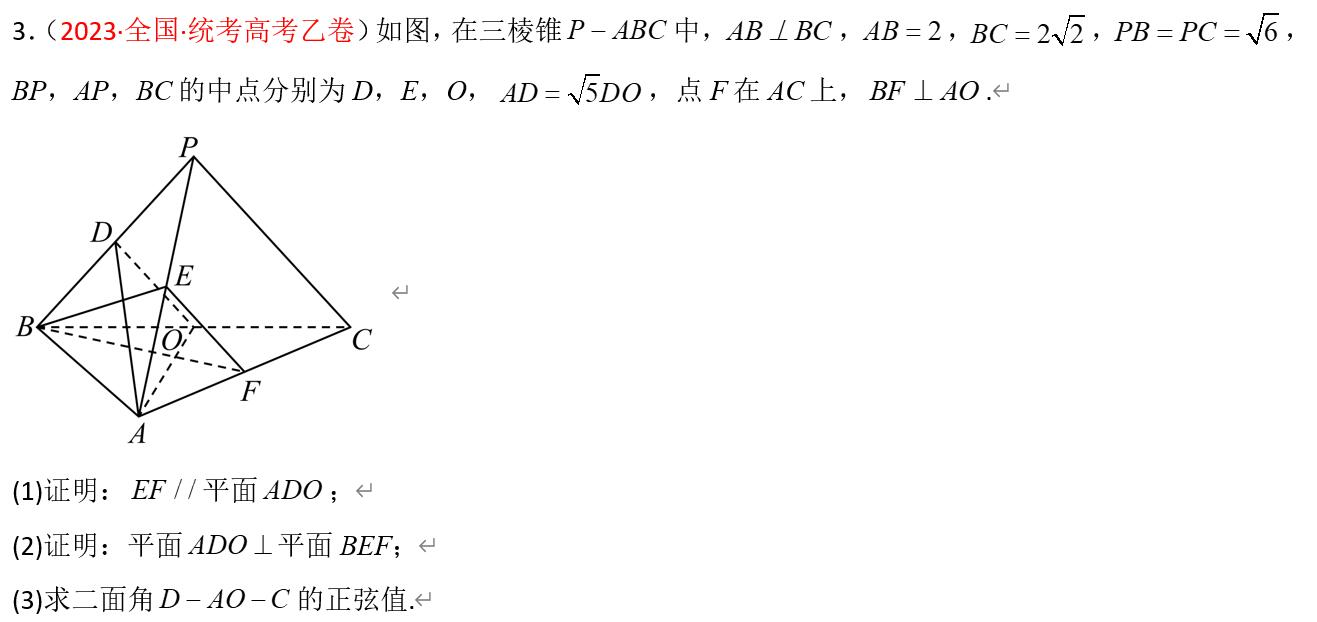
\includegraphics[scale=0.5]{./2023_yi.jpg}\\
Solution:\\
(1) 连接 $D E, O F$, 设 $A F=t A C$, \\
则 $\overrightarrow{B F}=\overrightarrow{B A}+\overrightarrow{A F}=(1-t) \overrightarrow{B A}+t \overrightarrow{B C}, \overrightarrow{A O}=-\overrightarrow{B A}+\frac{1}{2} \overrightarrow{B C},\\ \because B F \perp A O$, \\则 $\overrightarrow{B F} \cdot \overrightarrow{A O}=[(1-t) \overrightarrow{B A}+t \overrightarrow{B C}] \cdot\left(-\overrightarrow{B A}+\frac{1}{2} \overrightarrow{B C}\right)=(t-1) \overrightarrow{B A}^2+\frac{1}{2} t \overrightarrow{B C^2}=4(t-1)+4 t=0$,\\ 解得 $t=\frac{1}{2}$, 则 $F$ 为 $A C$ 的中点,\\ 由 $D, E, O, F$ 分别为 $P B, P A, B C, A C$ 的中点,\\ 于是 $D E / / A B, D E=\frac{1}{2} A B, O F / / A B, O F=\frac{1}{2} A B$, 即 $D E / / O F, D E=O F$,\\ 则四边形 $O D E F$ 为平行四边形, $E F / / D O, E F=D O$,\\ 又 $E F \not \subset$ 平面 $A D O, D O \subset$ 平面 $A D O$,\\ 所以 $E F / /$ 平面 $A D O$.\\
(2)法一:由(1)可知 $E F / / O D$, \\则 $A O=\sqrt{6}, D O=\frac{\sqrt{6}}{2}$, 得 $A D=\sqrt{5} D O=\frac{\sqrt{30}}{2}$,\\ 因此 $O D^2+A O^2=A D^2=\frac{15}{2}$, 则 $O D \perp A O$, 有 $E F \perp A O$,\\ 又 $A O \perp B F, B F \cap E F=F, B F, E F \subset$ 平面 $B E F$ ,\\
则有 $A O \perp$ 平面 $B E F$, \\又 $A O \subset$ 平面 $A D O$, \\所以平面 $A D O \perp$ 平面 $B E F$.\\
法二: 因为 $A B \perp B C$, 过点 $\mathrm{A}$ 作 $z$ 轴 $\perp$ 平面 $B A C$, 建立如图所示的空间直角坐标系,\\ $\therefore A(2,0,0),, B(0,0,0), C(0,2 \sqrt{2}, 0)$,\\
在 $\displaystyle\triangle B D A$ 中, $\displaystyle\cos \angle P B A=\frac{D B^2+A B^2-D A^2}{2 D B \cdot A B}=\frac{\frac{3}{2}+4-\frac{15}{2}}{2 \times 2 \times \frac{\sqrt{6}}{2}}=-\frac{1}{\sqrt{6}}$,\\
在 $\triangle P B A$ 中, $P A^2=P B^2+A B^2-2 P B \cdot A B \cos \angle P B A=6+4-2 \sqrt{6} \times 2 \times\left(-\frac{1}{\sqrt{6}}\right)=14$,\\
设 $P(x, y, z)$, 所以由 $\left\{\begin{array}{l}P A=\sqrt{14} \\ P B=\sqrt{6} \\ P C=\sqrt{6}\end{array}\right.$ 可得: $\left\{\begin{array}{l}(x-2)^2+y^2+z^2=14 \\ x^2+y^2+z^2=6 \\ x^2+(y-2 \sqrt{2})^2+z^2=6\end{array}\right.$,\\
可得: $x=-1, y=\sqrt{2}, z=\sqrt{3}$, 所以 $P(-1, \sqrt{2}, \sqrt{3})$,\\
则 $\displaystyle D\left(-\frac{1}{2}, \frac{\sqrt{2}}{2}, \frac{\sqrt{3}}{2}\right)$, 所以 $\displaystyle E\left(\frac{1}{2}, \frac{\sqrt{2}}{2}, \frac{\sqrt{3}}{2}\right), F(1, \sqrt{2}, 0)$,
$\displaystyle\overrightarrow{A O}=(-2, \sqrt{2}, 0), \overrightarrow{A D}=\left(-\frac{5}{2}, \frac{\sqrt{2}}{2}, \frac{\sqrt{3}}{2}\right)$\\
设平面 $A D O$ 的法向量为 $\overrightarrow{n_1}=\left(x_1, y_1, z_1\right)$,\\
则 $\left\{\begin{array}{l}\vec{n}_1 \cdot \overrightarrow{A O}=0 \\ \vec{n}_1 \cdot \overline{A D}=0\end{array}\right.$, 得 $\left\{\begin{array}{l}\displaystyle-2 x_1+\sqrt{2} y_1=0 \\ \displaystyle-\frac{5}{2} x_1+\frac{\sqrt{2}}{2} y_1+\frac{\sqrt{3}}{2} z_1=0\end{array}\right.$ ,\\
令 $x_1=1$, 则 $y_1=\sqrt{2}, z_1=\sqrt{3}$, 所以 $\overrightarrow{n_1}=(1, \sqrt{2}, \sqrt{3})$\\
$\displaystyle
\overrightarrow{B E}=\left(\frac{1}{2}, \frac{\sqrt{2}}{2}, \frac{\sqrt{3}}{2}\right), \overrightarrow{B F}=(1, \sqrt{2}, 0)
$\\
设平面 $B E F$ 的法向量为 $\overrightarrow{n_2}=\left(x_2, y_2, z_2\right)$,\\
则 $\displaystyle\left\{\begin{array}{l}\displaystyle\overrightarrow{n_2} \cdot \overrightarrow{B E}=0 \\ \displaystyle\overline{n_2} \cdot \overrightarrow{B F}=0\end{array}\right.$, 得 $\displaystyle\left\{\begin{array}{l}\displaystyle\frac{1}{2} x_2+\frac{\sqrt{2}}{2} y_2+\frac{\sqrt{3}}{2} z_2=0 \\\displaystyle x_2+\sqrt{2} y_2=0\end{array}\right.$,\\
令 $x_2=2$, 则 $y_2=-\sqrt{2}, z_2=0$, 所以 $\overrightarrow{n_2}=(2,-\sqrt{2}, 0)$,\\ $\overrightarrow{n_1} \cdot \overrightarrow{n_2}=2 \times 1+\sqrt{2} \times(-\sqrt{2})+0=0$,\\
所以平面 $A D O \perp$ 平面 $B E F$;\\
(3) 法- : 过点 $O$ 作 $O H / / B F$ 交 $A C$ 于点 $H$, 设 $A D \cap B E=G$, 由 $A O \perp B F$, 得 $H O \perp A O$, 且 $F H=\frac{1}{3} A H$,\\
又由 (2) 知, $O D \perp A O$, 则 $\angle D O H$ 为二面角 $D-A O-C$ 的平面角,\\
因为 $D, E$ 分别为 $P B, P A$ 的中点, \\
因此 $G$ 为 $\triangle P A B$ 的重心, 即有 $\displaystyle D G=\frac{1}{3} A D, G E=\frac{1}{3} B E$, \\
又 $F H=\frac{1}{3} A H$, 即有 $\displaystyle D H=\frac{3}{2} G F$, $\displaystyle\cos \angle A B D=\frac{4+\frac{3}{2}-\frac{15}{2}}{2 \times 2 \times \frac{\sqrt{6}}{2}}=\frac{4+6-P A^2}{2 \times 2 \times \sqrt{6}}$, 解得 $P A=\sqrt{14}$, \\
同理得 $B E=\frac{\sqrt{6}}{2}$, 于是 $B E^2+E F^2=B F^2=3$, 即有 $B E \perp E F$,\\
则 $\displaystyle G F^2=\left(\frac{1}{3} \times \frac{\sqrt{6}}{2}\right)^2+\left(\frac{\sqrt{6}}{2}\right)^2=\frac{5}{3}$,从而 $\displaystyle G F=\frac{\sqrt{15}}{3}, D H=\frac{3}{2} \times \frac{\sqrt{15}}{3}=\frac{\sqrt{15}}{2}$, \\
在 $\displaystyle\triangle D O H$ 中, $\displaystyle O H=\frac{1}{2} B F=\frac{\sqrt{3}}{2}, O D=\frac{\sqrt{6}}{2}, D H=\frac{\sqrt{15}}{2}$,\\
于是 $\displaystyle\cos \angle D O H=\frac{\frac{6}{4}+\frac{3}{4}-\frac{15}{4}}{2 \times \frac{\sqrt{6}}{2} \times \frac{\sqrt{3}}{2}}=-\frac{\sqrt{2}}{2}, \sin \angle D O H=\sqrt{1-\left(-\frac{\sqrt{2}}{2}\right)^2}=\frac{\sqrt{2}}{2}$, \\所以二面角 $D-A O-C$ 的正弦值为 $\displaystyle\frac{\sqrt{2}}{2}$.\\
法二: 平面 $A D O$ 的法向量为 $\vec{n}_1=(1, \sqrt{2}, \sqrt{3})$, 平面 $A C O$ 的法向量为 $\bar{n}_3=(0,0,1)$,\\
$\begin{aligned}
	&\text{所以}\cos\left\langle\overrightarrow{n_1},\overrightarrow{n_3}\right\rangle=\frac{n_1\cdot n_3}{\left|\overrightarrow{n_1}\right|\cdot\left|\overrightarrow{n_3}\right|}=\frac{\sqrt{3}}{\sqrt{1+2+3}}=\frac{\sqrt{2}}2\text{ , } \\
	&\text{因为}\left\langle\overrightarrow{n_1},\overrightarrow{n_3}\right\rangle\in\left[0,\pi\right]\text{,所以}\sin\left\langle\overrightarrow{n_1},\overrightarrow{n_3}\right\rangle=\sqrt{1-\cos^2\left\langle\overrightarrow{n_1},\overrightarrow{n_3}\right\rangle}=\frac{\sqrt{2}}2\text{,台} \\
	&\text{故二面角}D-AO-C\text{ 的正弦值为}\frac{\sqrt{2}}2.
	

\end{aligned}$\\
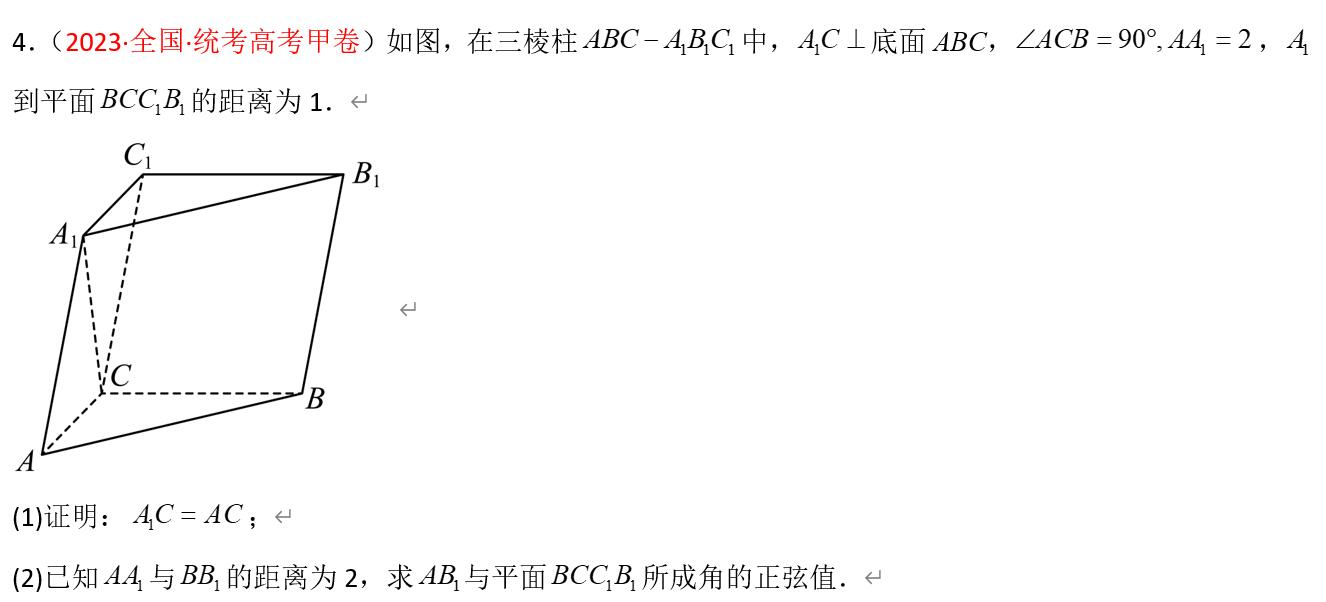
\includegraphics[scale=0.5]{./2023_jia.jpg}\\
Solution:\\
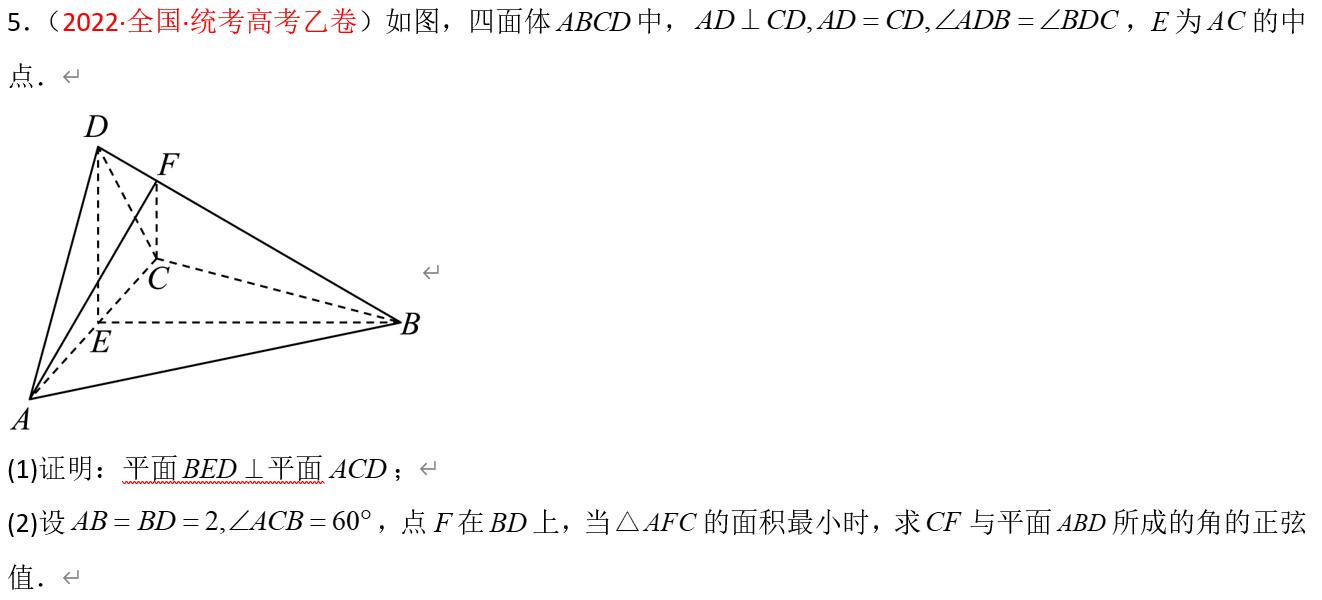
\includegraphics[scale=0.5]{./2022_yi.jpg}\\
Solution:\\
\end{document}
